\documentclass{jsarticle}
\usepackage[dvipdfmx]{graphicx}
\usepackage{bm}
\usepackage{amsmath}
\usepackage{amssymb}
\usepackage{amsfonts}
\usepackage{comment}
\usepackage{listings}
\usepackage{cases}
\lstset{
    basicstyle={\ttfamily},
    identifierstyle={\small},
    commentstyle={\smallitshape},
    keywordstyle={\small\bfseries},
    ndkeywordstyle={\small},
    stringstyle={\small\ttfamily},
    frame={tb},
    breaklines=true,
    columns=[l]{fullflexible},
    numbers=left,
    xrightmargin=0zw,
    xleftmargin=3zw,
    numberstyle={\scriptsize},
    stepnumber=1,
    numbersep=1zw,
    lineskip=-0.5ex,
    keepspaces=true,
    language=c
}
\renewcommand{\lstlistingname}{リスト}
\makeatletter
\newcommand{\figcaption}[1]{\def\@captype{figure}\caption{#1}}
\newcommand{\tblcaption}[1]{\def\@captype{table}\caption{#1}}
\makeatother

\title{科学技術英語 英文読解課題}
\author{Ec5 24番 平田 蓮}
\date{}

\begin{document}
\maketitle
\section*{付録A 発展的なNumPy}
    この付録では、配列計算のためのNumPyライブラリをより深く掘り下げていきます。
    これにはndarray型の内部の詳細や、より高度な配列操作とそのアルゴリズムが含まれます。

    この付録は雑多な内容を含んでおり続けて読む必要はありません。

    \subsection*{A.1 ndarrayオブジェクトの内部構造}
        NumPyのndarrayは、同じ型のデータのブロックを
        (連続か区切られているかにかかわらず)
        多次元配列オブジェクトとして提供します。
        データ型(dtype)は、データが浮動小数点、整数、真偽値、
        あるいはこれまで見てきた他の型のどれであるかを決定します。

        ndarrayを柔軟にしている理由の一つに、
        すべての配列オブジェクトがデータをブロック区切りでみていることがあります。
        例えば配列に対する参照\verb|arr[::2, ::-1]|がデータを一切コピー
        していないことを不思議に思うかもしれません。
        その理由は、ndarrayは単なるデータとその型の集まりではなく、
        配列がメモリ内をさまざまなステップサイズで移動できるようにする「ストライド」
        情報を持っているからです。
        より正確に言うと、ndarrayの内部は以下のような構成になっています。

        \begin{itemize}
            \item RAMやメモリマップ内にあるデータの集まりへのポインタ
            \item 配列内の一定個数のデータの型
            \item 配列の形を表すタプル
            \item 各次元に沿って要素を一つ進めるために遷移するバイト数(整数値)のタプル
        \end{itemize}

        図\ref{fig:A-1}は、ndarrayの内部構造を示す模式図です。

        \begin{figure}[h]
            \centering
            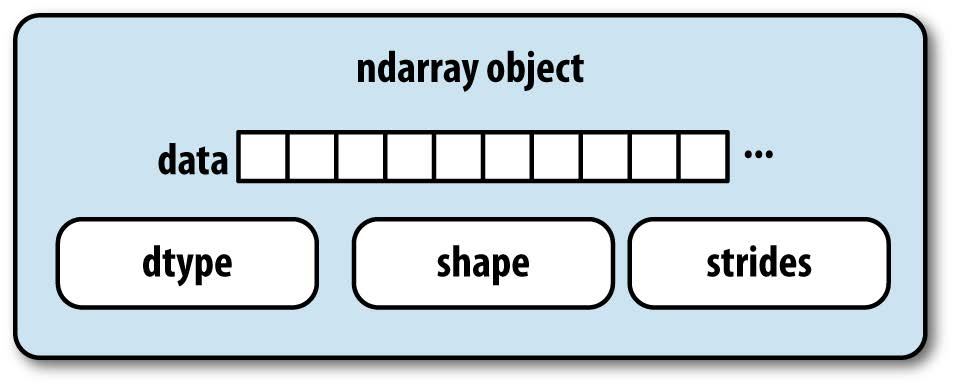
\includegraphics[width=10cm]{images/A-1.jpg}
            \caption{NumPyのndarrayオブジェクト}
            \label{fig:A-1}
        \end{figure}

        例えば、10 $\times$ 5の配列は\verb|(10, 5)|の形を持っています。

        \begin{lstlisting}
np.ones((10, 5)).shape # (10, 5)\end{lstlisting}

        float64(8バイト)型の典型的な3$\times$4$\times$5配列は、
        \verb|(160, 40, 8)|のストライドを持っています。
        (一般的に特定の軸のストライドが大きいほど、
        その軸に沿って計算を行うコストが高くなるので、
        ストライドについて知っておくと便利です。)

        \begin{lstlisting}
np.ones((3, 4, 5), dtype=np.float64).strides # (160, 40, 8)\end{lstlisting}

        典型的なNumPyユーザーが配列のストライドに興味を持つことは稀ですが、
        ストライドは0配列をコピー、構築するための重要な要素です。
        ストライドには負の値を設定することもでき、
        配列をメモリ上で逆向きに移動させることができます
        (例えば、\verb|obj[::-1]|や\verb|obj[:, ::-1]|
        のようなスライスがこれに該当します)。

        \subsubsection*{NumPyのdtypeの階層構造}
            配列の中に整数、浮動小数点数、文字列、
            Pythonオブジェクトが含まれているかどうかのチェックが
            必要なコードがあるかもしれません。
            浮動小数点数には複数の型(float16~float128)があるため、
            その配列のdtypeが型一覧の中にあるかどうかをチェックするのは非常に冗長です。
            幸い、dtypeには\verb|np.integer|や\verb|np.floating|
            などのスーパークラスがあり、
            \verb|np.issubdtype()|と組み合わせて使用することができます。

            \begin{lstlisting}
ints = np.ones(10, dtype=np.uint16)
floats = np.ones(10, dtype=np.float32)

np.issubdtype(ints.dtype, np.integer) # True
np.issubdtype(floats.dtype, np.floating) # True\end{lstlisting}

            特定のdtypeの親クラスをすべて見るには、
            その型の\verb|mro|メソッドを呼び出します。

            \begin{lstlisting}
np.float64.mro() # [numpy.float64, numpy.floating, numpy.inexact, numpy.number, numpy.generic, float, object]\end{lstlisting}

            図\ref{fig:A-2}は、dtypeの階層と親、サブクラスの関係を示したものです。

            \begin{figure}[h]
                \centering
                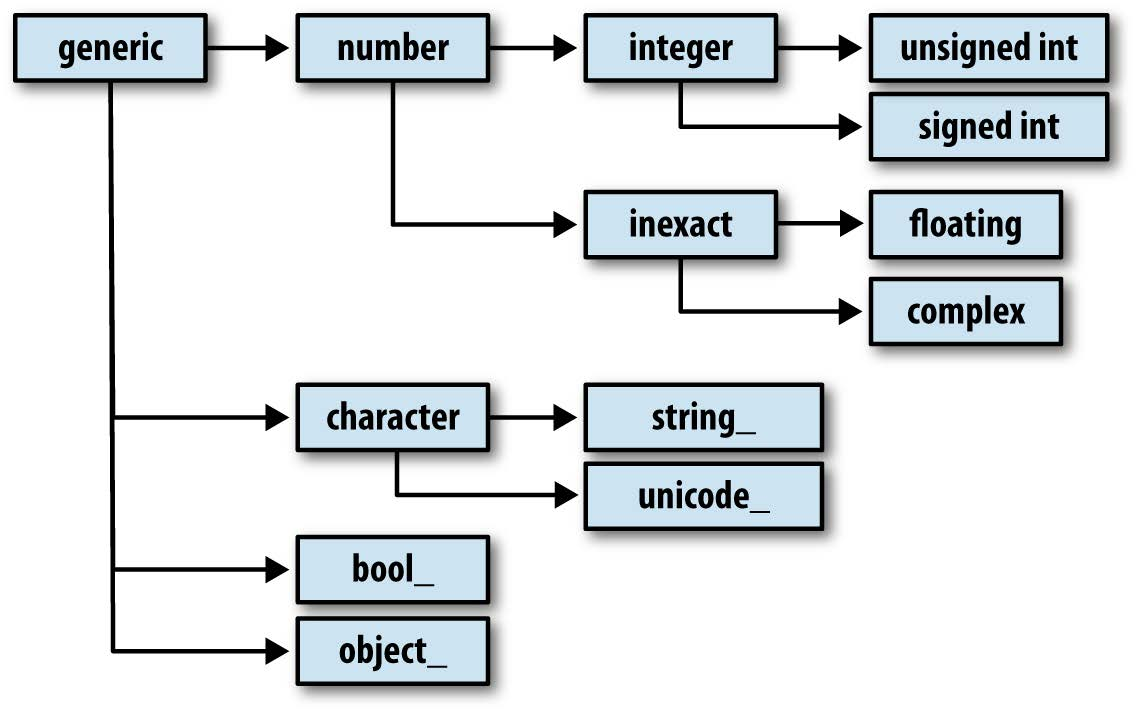
\includegraphics[width=10cm]{images/A-2.jpg}
                \caption{NumPyのdtypeの階層構造}
                \label{fig:A-2}
            \end{figure}

    \subsection*{A.2 発展的な配列操作}
        配列を扱う方法には、インデックス、スライス、ブーリアン
        のサブセットといった洒落た方法以外のものもたくさんあります。
        データ分析アプリケーションの大部分はpandasの高レベル関数で処理されますが、
        既存のライブラリにはないデータアルゴリズムを書かなければならない
        場合もあるでしょう。

        \subsubsection*{配列の変形}
            多くの場合、データを一切コピーせずに
            配列を他の形へ変形できます。
            そのためには、配列の\verb|reshape|メソッドに新しい形を表す
            タプルを渡します。
            例えば、ある値を持つ一次元の配列を行列に並べ替えたいとします。
            (結果は図\ref{fig:A-3}の通りです。)

            \begin{lstlisting}
arr = np.arange(8) # [0, 1, 2, 3, 4, 5, 6, 7]
arr.reshape((4, 2)) # [[0, 1], [2, 3], [4, 5], [6, 7]]\end{lstlisting}

            \begin{figure}[h]
                \centering
                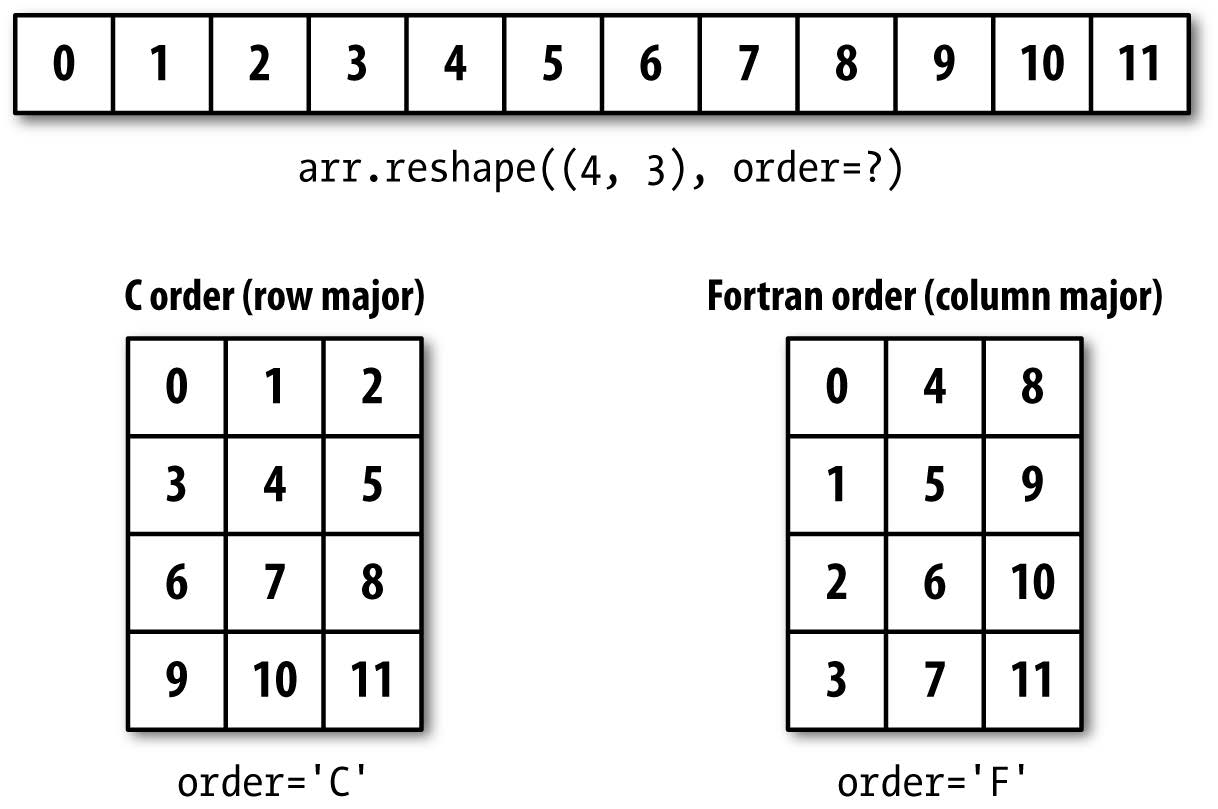
\includegraphics[width=10cm]{images/A-3.jpg}
                \caption{C(行優先)順序とFortran(列優先)順序での変形}
                \label{fig:A-3}
            \end{figure}

            多次元配列は次のように変形することもできます。

            \begin{lstlisting}
arr.reshape((4, 2)).reshape((2, 4)) # [[0, 1, 2, 3], [4, 5, 6, 7]]\end{lstlisting}

            形を表す次元数のうち、一つは-1にすることが可能で、
            その場合、その次数はデータから推測されます。

            \begin{lstlisting}
arr = np.arange(15)
arr.reshape((5, -1)) # [[ 0, 1, 2], [ 3, 4, 5], [ 6, 7, 8], [ 9, 10, 11], [12, 13, 14]]\end{lstlisting}

            配列の\verb|shape|属性はタプルであるので、\verb|reshape()|に渡すことも可能です。

            \begin{lstlisting}
other_arr = np.ones((3, 5))
other_arr.shape # (3, 5)
arr.reshape(other_arr.shape) # [[ 0, 1, 2, 3, 4], [ 5, 6, 7, 8, 9], [10, 11, 12, 13, 14]]\end{lstlisting}

            一次元から高次元への変形の逆の操作は一般的に
            フラットニングやラベリングと呼ばれます。

            \begin{lstlisting}
arr = np.arange(15).reshape((5, 3)) # [[ 0, 1, 2], [ 3, 4, 5], [ 6, 7, 8], [ 9, 10, 11], [12, 13, 14]]
arr.ravel() # [ 0, 1, 2, 3, 4, 5, 6, 7, 8, 9, 10, 11, 12, 13, 14]\end{lstlisting}

            \verb|ravel()|は変形後の値が隣接している場合、元の値をコピーしません。
            \verb|flatten|メソッドは常にデータのコピーを返すという点を除いて、
            \verb|ravel|と同じ動作をします。

            \begin{lstlisting}
arr.flatten() # [ 0, 1, 2, 3, 4, 5, 6, 7, 8, 9, 10, 11, 12, 13, 14]\end{lstlisting}

            データは違う順序で変形したり、ラベリングしたりすることができます。
            これは、NumPyの新規ユーザーにとっては少しニュアンスの異なるトピック
            であるため、次のサブトピックです。
\end{document}